% =============================================================
%  DC Fault Ride-Through
%  DC line fault recovery of a half-bridge MMC symmetrical monopole,
%  on the record of the Pugalur--Thrissur link (±320 kV, 2 x 1000 MW):
%  specified recovery times, switchgear, the recovery sequence,
%  commissioning and field records, fault zones, STATCOM changeover,
%  ratings and the design alternatives.
%  Sources: [24] Westerweller et al., CIGRE 2022, paper 10466;
%           [25] Kumar et al., CIGRE 2026, paper 10563.
%  Figures: switchgear single-line, fault zones and the recovery
%  timeline as inline TikZ; the recorded voltages and currents are the
%  oscillograms of the two papers, extracted unchanged from the PDFs
%  (pdfimages) into fig/ -- w2022_* from [24], k2026_* from [25]. The
%  file names carry the figure number of the source.
% =============================================================
\section{DC Fault Ride-Through}
\label{sec:dc-fault}

A fault on the DC side of a VSC HVDC link interrupts the power transfer. On a
link whose DC circuit is at least partly an overhead line, most of these
faults are temporary flashovers --- lightning, pollution, vegetation --- and
the link is expected to clear the fault and restore transmission on its own,
as an AC line does by auto-reclosure. This chapter describes that behaviour
for a half-bridge MMC in a symmetrical monopole, on the record of the
Pugalur--Thrissur link in India. The supplier's description of the
design~[24] and the operator's evaluation of five years of fault
records~[25] are the sources; every number in this chapter is theirs.

The term used throughout is the one of the project specification: a
\emph{DC line fault recovery sequence}, a defined series of restart attempts
after a fault on the DC line. The expression \emph{DC fault ride-through} in
the chapter title names the same behaviour from the point of view of the AC
network.

\subsection{Reference project}
\label{sec:dc-fault-project}

The Pugalur--Thrissur link connects Pugalur (Tamil Nadu) and North Thrissur
(Kerala) with two independent symmetrical monopoles of 1000\,MW each, at
$\pm$320\,kV, bidirectional, with half-bridge MMC converters and a reactive
power capability of $\pm$1100\,Mvar~[25]. The DC circuit is a hybrid of
150\,km overhead line and 28\,km XLPE cable; a transition station 28\,km
from Thrissur joins the two~[25] (the project map in~[24] gives 143\,km and
32\,km). At Pugalur the link shares the 400\,kV AC bus with the
$\pm$800\,kV, 6000\,MW LCC link from Raigarh. It was commissioned in 2021.
Table~\ref{tab:dcf-system} lists the system parameters the recovery
performance was specified against.

\begin{table}[!ht]
  \centering
  \begin{tabular}{@{}l l r r@{}}
    \toprule
    \textbf{Parameter} & & \multicolumn{1}{c}{\textbf{Pugalur}}
      & \multicolumn{1}{c}{\textbf{Thrissur}} \\
    \midrule
    AC voltage, max./min.          & kV   & 440 / 360 & 440 / 360 \\
    AC frequency, max./min.        & Hz   & 52.5 / 47.5 & 52.5 / 47.5 \\
    Negative-sequence voltage      & \%   & 1.5 & 1.5 \\
    Short-circuit power, max./min. & MVA  & 36\,400 / 390 & 36\,400 / 390 \\
    DC voltage, pole to pole       & kV   & \multicolumn{2}{c}{640} \\
    DC current                     & A    & \multicolumn{2}{c}{1563} \\
    Sub-module type                &      & \multicolumn{2}{c}{half-bridge} \\
    \bottomrule
  \end{tabular}
  \caption{System parameters of the Pugalur--Thrissur VSC HVDC link~[25]}
  \label{tab:dcf-system}
\end{table}

\subsection{Fault behaviour of the half-bridge converter}
\label{sec:dc-fault-behaviour}

A blocked half-bridge MMC is an uncontrolled diode rectifier between the AC
network and the DC circuit. Blocking the converter therefore neither
interrupts the fault current nor de-energises the DC circuit: the AC network
keeps feeding the fault through the diodes until the AC circuit breakers of
both stations open~[24]. Opening the AC circuit breakers is thus a mandatory
part of every DC fault clearing on this converter type, and the mechanical
switchgear of Section~\ref{sec:dc-fault-switchgear} sets the pace of the
recovery.

The symmetrical monopole is the DC equivalent of an ungrounded AC network.
Its ground reference is a high-impedance star-point unit, which grades the
two pole voltages against ground, so the two fault types behave
differently~[24]:

\begin{itemize}[itemsep=0.2em]
  \item \textbf{Pole-to-ground fault.} The high grounding impedance limits
        the fault current to the discharge of the faulted pole and the
        charging of the healthy one. The healthy pole, however, rises
        towards the full pole-to-pole voltage: the records of~[25] show up
        to 600\,kV on a $\pm$320\,kV link, limited by the arresters. The
        overvoltage persists after the AC circuit breakers open, because the
        cable section stores the charge, and has to be removed by a
        discharge unit before the restart.
  \item \textbf{Pole-to-pole fault.} There is no overvoltage, but a fault
        current fed by the diode rectifiers of both stations. After the AC
        circuit breakers open, this current freewheels through the converter
        diodes, driven by the energy in the converter reactors and the DC
        circuit, and decays with the $L/R$ time constant of the fault loop.
        With no fault impedance the decay takes up to 500\,ms~[24]. The
        deionisation time starts only when the current has reached zero.
\end{itemize}

The fault detection and the blocking are independent of the fault location:
the IGBTs have to be switched off within microseconds, before the current
exceeds their turn-off capability, which rules out any selective decision at
that stage~[24]. Selectivity --- in which zone the fault lies and whether a
restart is permitted --- is decided afterwards, during the fault clearing,
Section~\ref{sec:dc-fault-zones}.

\subsection{Specified recovery performance}
\label{sec:dc-fault-spec}

The technical specification of the project defines the recovery as a
sequence of up to three restart attempts, each with its own target state
and time limit~[24], [25]:

\begin{enumerate}[itemsep=0.2em]
  \item \textbf{First restart} at the pre-fault direct voltage and power
        transfer, within 1.5\,s of a pole-to-ground fault and 1.8\,s of a
        pole-to-pole fault, both including fault clearing and cable
        discharge.
  \item \textbf{Second restart} at a reduced direct voltage, with the power
        curtailed accordingly. Its duration is governed by the on-load
        tap-changer and the recharging of the switchgear drives, and is
        specified only as slow, above 10\,s.
  \item \textbf{Changeover to STATCOM operation} if the second restart fails:
        the DC line is de-energised permanently and both converter stations
        reconfigure to reactive power support of the AC network, again above
        10\,s.
\end{enumerate}

The STATCOM requirement comes from the AC network: the loss of the
transmission changes the load flows and raises the need for reactive power,
and the converter supplies it without additional FACTS equipment. The same
requirement applies after a permanent fault in the DC cable or in one of the
converter stations~[24].

A fault within 15\,min of the previous one counts as a consecutive fault of
the same sequence, and only the remaining attempts are made; after 15\,min
without a fault the sequence is complete and the next fault opens a new one
with all three attempts. Three such sequences have to be possible within
45\,min~[24], [25]. As the project has two parallel links, the specification
also requires the active power of the faulted link to be transferred to the
healthy one, as far as its rating allows, within 80\,ms~[24].
Table~\ref{tab:dcf-spec} collects the times.

\begin{table}[!ht]
  \centering
  \begin{tabularx}{\linewidth}{@{}>{\raggedright\arraybackslash}X l@{}}
    \toprule
    \textbf{Step} & \multicolumn{1}{c}{\textbf{Specified time}} \\
    \midrule
    First restart, pole-to-ground fault (incl.\ fault clearing and
      cable discharge) & $< 1.5$\,s \\
    First restart, pole-to-pole fault & $< 1.8$\,s \\
    Second restart at reduced direct voltage & $> 10$\,s (tap-changer, drive recharge) \\
    Changeover to STATCOM operation & $> 10$\,s \\
    Power compensation by the parallel link & $< 80$\,ms \\
    Consecutive fault & within 15\,min of the previous one \\
    Recovery sequences to be withstood & 3 within 45\,min \\
    \bottomrule
  \end{tabularx}
  \caption{Recovery performance specified for the Pugalur--Thrissur
           link~[24], [25]}
  \label{tab:dcf-spec}
\end{table}

\subsection{Switchgear of the recovery sequence}
\label{sec:dc-fault-switchgear}

Figure~\ref{fig:dcf-switchgear} shows the single-line diagram of one
converter station with the switchgear the recovery sequence operates~[24],
[25]. Four devices take part:

\begin{itemize}[itemsep=0.2em]
  \item \textbf{AC circuit breaker.} Clears the fault by separating the
        diode rectifier from the AC network, and re-energises the interface
        transformer and the converter at the restart.
  \item \textbf{Insertion resistor and bypass switch.} The insertion
        resistor is in series with the network terminals of the interface
        transformer and is bypassed in normal operation. For the restart the
        bypass switch is opened before the circuit breaker closes, so the
        DC circuit is charged through the resistor and the diodes. The
        resistor limits the inrush of the diodes and, if the fault
        persists, the uncontrolled fault current. Once the charging current
        has decayed the bypass switch closes and the converter is
        deblocked.
  \item \textbf{Discharge unit.} One per pole: a fast-acting grounding
        switch in series with a damping resistor. It removes the trapped
        charge of the healthy pole after a pole-to-ground fault, and is
        closed only for that purpose. The resistance is chosen well above
        the surge impedance of the DC circuit so that the discharge does not
        launch travelling waves of its own~[24]. At Pugalur--Thrissur the
        discharge is led by the Thrissur station, the Pugalur unit being
        the backup~[25].
  \item \textbf{DC disconnect switches.} Slow devices that separate a
        converter station from the DC circuit for STATCOM operation. Their
        operating time, 15\,s and more, is one of the two terms that set the
        changeover time of Section~\ref{sec:dc-fault-statcom}.
\end{itemize}

\begin{figure}[!ht]
  \centering
  \begin{tikzpicture}[font=\small, >=Latex, line width=0.7pt,
      sw/.style={line width=0.7pt},
      res/.style={draw, minimum width=0.8cm, minimum height=0.3cm, inner sep=0pt}]
    % AC network
    \draw (0,0) -- (0.6,0);
    \fill (0,0) circle (0.05);
    \draw (0.3,-0.2) -- (0.5,0.2) (0.4,-0.2) -- (0.6,0.2) (0.5,-0.2) -- (0.7,0.2);
    \node[below, font=\footnotesize] at (0.3,-0.25) {AC network};
    % circuit breaker
    \draw (0.7,0) -- (1.3,0);
    \draw[sw] (1.3,0) -- (1.9,0.3);
    \draw (1.95,0) -- (2.6,0);
    \draw (1.55,-0.35) rectangle (1.75,-0.15);
    \node[below, align=center, font=\footnotesize] at (1.65,-0.45) {circuit\\breaker};
    % insertion resistor with bypass switch
    \draw (2.6,0) -- (2.6,0.6) -- (3.3,0.6);
    \node[res] at (3.7,0.6) {};
    \draw (4.1,0.6) -- (4.8,0.6) -- (4.8,0);
    \node[above, font=\footnotesize] at (3.7,0.75) {insertion resistor};
    \draw (2.6,0) -- (3.3,0);
    \draw[sw] (3.3,0) -- (3.9,0.3);
    \draw (3.95,0) -- (4.8,0);
    \draw (3.55,-0.35) rectangle (3.75,-0.15);
    \node[below, align=center, font=\footnotesize] at (3.65,-0.45) {bypass\\switch};
    % interface transformer
    \draw (4.8,0) -- (5.6,0);
    \draw (5.95,0) circle (0.35);
    \draw (6.45,0) circle (0.35);
    \draw (6.8,0) -- (7.6,0);
    \node[below, align=center, font=\footnotesize] at (6.2,-0.45) {interface\\transformer};
    % converter
    \draw (7.6,-0.9) rectangle (9.4,0.9);
    \draw (7.6,-0.9) -- (9.4,0.9);
    \node[font=\footnotesize] at (8.0,0.45) {$\approx$};
    \node[font=\footnotesize] at (9.0,-0.45) {$=$};
    \node[below, align=center, font=\footnotesize] at (8.5,-0.95) {HVDC\\converter};
    % DC terminals
    \draw (9.4,0.6) -- (9.4,1.6) -- (11.8,1.6);
    \draw (9.4,-0.6) -- (9.4,-1.6) -- (11.8,-1.6);
    \fill (11.8,1.6) circle (0.05);
    \fill (11.8,-1.6) circle (0.05);
    \node[right, font=\footnotesize] at (11.85,1.6) {$+$};
    \node[right, font=\footnotesize] at (11.85,-1.6) {$-$};
    % discharge unit (positive pole): switch and resistor down to ground
    \fill (10.4,1.6) circle (0.04);
    \draw (10.4,1.6) -- (10.4,1.35);
    \draw[sw] (10.4,1.35) -- (10.65,0.9);
    \draw (10.4,0.85) -- (10.4,0.65);
    \node[res, rotate=90] at (10.4,0.25) {};
    \draw (10.4,-0.15) -- (10.4,-0.35);
    \draw (10.2,-0.35) -- (10.6,-0.35) (10.27,-0.45) -- (10.53,-0.45) (10.34,-0.55) -- (10.46,-0.55);
    \draw (10.65,1.2) rectangle (10.85,1.0);
    % discharge unit (negative pole): switch and resistor up to ground
    \fill (11.3,-1.6) circle (0.04);
    \draw (11.3,-1.6) -- (11.3,-1.35);
    \draw[sw] (11.3,-1.35) -- (11.55,-0.9);
    \draw (11.3,-0.85) -- (11.3,-0.65);
    \node[res, rotate=90] at (11.3,-0.25) {};
    \draw (11.3,0.15) -- (11.3,0.35);
    \draw (11.1,0.35) -- (11.5,0.35) (11.17,0.45) -- (11.43,0.45) (11.24,0.55) -- (11.36,0.55);
    \draw (11.55,-1.2) rectangle (11.75,-1.0);
    \node[right, align=left, font=\footnotesize] at (11.9,0.0) {discharge\\units};
  \end{tikzpicture}
  \caption{Switchgear of one converter station taking part in the DC line
           fault recovery, after~[24]: AC circuit breaker, insertion resistor
           with bypass switch, interface transformer, converter and one
           discharge unit per pole}
  \label{fig:dcf-switchgear}
\end{figure}

\subsection{Recovery sequence}
\label{sec:dc-fault-sequence}

The first restart after a pole-to-ground fault on the overhead line runs in
eight steps, coordinated between the two converter stations and the
transition station over the HVDC telecontrol; without telecontrol the
sequence cannot start~[25].

\begin{enumerate}[itemsep=0.2em]
  \item \textbf{Fault isolation.} The converters block on fault detection
        and the AC circuit breakers of both stations open. Until they open,
        the fault current flows through the diode path.
  \item \textbf{Fault current decay.} With the breakers open the fault
        current decays with the $L/R$ time constant of the loop, set mainly
        by the star-point units. The overvoltage of the healthy pole, limited
        by the arresters, discharges slightly.
  \item \textbf{Discharge and deionisation.} The discharge unit of the lead
        station closes and removes the charge of the healthy pole; the
        bypass switch of the insertion resistor opens. The arc at the fault
        location deionises.
  \item \textbf{Condition verification.} Both stations check breaker and
        bypass-switch positions, arm, DC and star-point currents and DC
        voltages against their thresholds.
  \item \textbf{Tap-changer adjustment.} Only for a restart at reduced
        voltage: the tap-changers move to the start position given by the
        sequence counter.
  \item \textbf{Restart initiation.} The restart release closes the AC
        circuit breaker of the rectifier station first, then of the inverter
        station.
  \item \textbf{Passive charging.} The DC circuit charges through the
        insertion resistor and the diodes. The build-up of the voltages and
        the decay of the charging current confirm the integrity of the DC
        circuit before the resistor is bypassed or the converter is
        deblocked~[24]. Since the sub-module capacitors are still charged,
        this step is shorter than a cold start.
  \item \textbf{Converter deblocking.} The converters deblock and ramp to the
        reference direct voltage. The rectifier station restores its reactive
        power first; the inverter station then restores active and reactive
        power to the pre-fault values.
\end{enumerate}

Figure~\ref{fig:dcf-timing} gives the durations of the four phases as the
operator reports them from the fault records~[25]. The recovery from a
pole-to-pole fault omits the discharge unit, since there is no trapped
charge, but has to wait for the freewheeling current to reach zero before
the deionisation time starts, Section~\ref{sec:dc-fault-records-pp}.

\begin{figure}[!ht]
  \centering
  \begin{tikzpicture}[font=\footnotesize, >=Latex,
      ph/.style={draw=atBorderStrong, line width=0.6pt, minimum height=3.9cm,
                 text width=2.55cm, align=left, inner sep=4pt, anchor=north west}]
    \node[ph, fill=atBgSubtle, minimum width=2.9cm] (a) at (0,0)
      {\textbf{Fault detection and converter block}\\[2pt]
       fault detection\\ converter block\\ AC circuit breaker opens\\
       fault current decays ($L/R$)};
    \node[ph, fill=atBgSubtle, minimum width=2.9cm] (b) at (3.0,0)
      {\textbf{Deionisation}\\[2pt]
       discharge unit closes\\ healthy pole discharges\\ fault arc deionises\\
       bypass switch opens};
    \node[ph, fill=atBgSubtle, minimum width=2.9cm] (c) at (6.0,0)
      {\textbf{Recovery}\\[2pt]
       AC circuit breaker closes\\ passive charging through the insertion resistor\\
       bypass switch closes\\ deblock, voltage build-up};
    \node[ph, fill=atBgSubtle, minimum width=2.9cm] (d) at (9.0,0)
      {\textbf{Power transfer}\\[2pt]
       power ramp\\ rebalancing with the parallel link};
    \foreach \n/\t in {a/200--250\,ms, b/250--400\,ms, c/550--580\,ms, d/175\,ms} {
      \draw[<->, atAccentFg, line width=0.7pt]
        ([yshift=0.25cm]\n.north west) -- ([yshift=0.25cm]\n.north east)
        node[midway, above, text=atFg] {\t};
    }
    \draw[->, line width=0.7pt] (0,-4.2) -- (12.0,-4.2) node[right] {$t$};
    \draw (0,-4.3) -- (0,-4.1) node[below=0.2cm] {$t_0$};
  \end{tikzpicture}
  \caption{Phases and durations of the first restart after a pole-to-ground
           fault on the DC overhead line, from the fault records of the
           Pugalur--Thrissur link~[25]}
  \label{fig:dcf-timing}
\end{figure}

\subsection{Recorded recoveries}
\label{sec:dc-fault-records}

\subsubsection{Pole-to-ground fault}
\label{sec:dc-fault-records-pg}

The commissioning record in~[24] shows a first restart with both links at
about 50\,\% active and reactive load and the fault on the positive pole.
The converters of the faulted link block at the fault instant $t_0$ and the
healthy link takes over the power within the specified time. The negative
pole is discharged at $t_0 + 180$\,ms, the circuit breaker of station~A
closes and passive charging starts at $t_0 + 520$\,ms, the bypass switch
closes at $t_0 + 700$\,ms with the deblocking of station~A, and station~B
deblocks at $t_0 + 915$\,ms and restores its reactive power. The active power
sharing between the two links is then restored with a long time constant, so
that the AC network sees no second disturbance; this slow return applies only
to the share the healthy link took over, and a share it could not take over
is restored immediately after deblocking~[24]. Figure~\ref{fig:dcf-pg-record}
is that record: the pole voltages $U_{dHP}$, $U_{dHN}$, the pole currents
$I_{dHP}$, $I_{dHN}$, the active power of the two links and their sum, and
the reactive power of the two links at each station. The negative pole
holds about $-580$\,kV until the discharge unit closes, and the active
power of link~2 (red) steps up to carry the total while link~1 (blue)
recovers.

\begin{figure}[!ht]
  \centering
  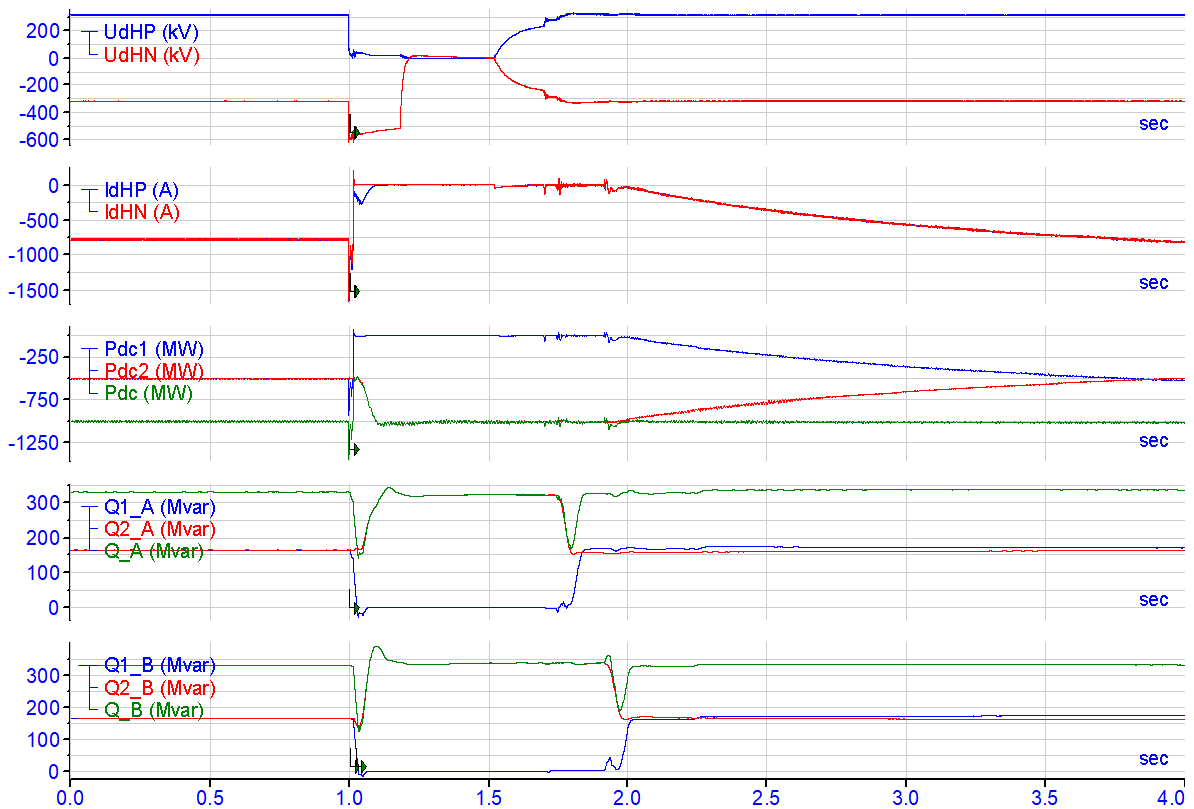
\includegraphics[width=\linewidth]{dc-fault-ride-through/fig/w2022_fig2_pg_recovery.png}
  \caption{Commissioning record of the first restart after a single
           pole-to-ground fault on the positive pole, both links at about
           50\,\% load; from top: pole voltages, pole currents, active power
           of link~1, link~2 and total, reactive power of both links at
           station~A and at station~B. Reproduced from~[24], Figure~2}
  \label{fig:dcf-pg-record}
\end{figure}

Table~\ref{tab:dcf-events} lists the three pole-to-ground faults the
operator evaluated from the transient fault recorder at Pugalur after five
years of service, together with the dynamic performance study case the
control design was validated against~[25]. The three field events share the
same sequence: the healthy pole rises to 600\,kV and is discharged until
$t_0 + 250$\,ms, the deionisation takes about 280\,ms, zone identification
and the reconfiguration request fall into these two intervals, the circuit
breaker recloses with the insertion resistor in circuit for about 200\,ms,
and the converter deblocks between $t_0 + 860$\,ms and $t_0 + 930$\,ms.
Power is restored to the pre-fault level within 2\,s in each case, and the
parallel link carries the power in the meantime. The simulated case at rated
power deblocks within 800\,ms. All recorded first restarts succeeded, and all
lie within the specified 1.5\,s~[25].

Figure~\ref{fig:dcf-pg-tfr} is the transient fault record of the first
event, at 400\,MW on link~1. The positive pole is the healthy one here and
rises to 600\,kV at the fault; the cursors mark 0.722\,s from the fault to
the reclosing of the circuit breaker, 0.193\,s of charging through the
insertion resistor, and 0.932\,s to deblocking. The binary channels below
the analogue traces show the blocking, the zone identification
(\emph{ZONE = DC OHL}), the reconfiguration request and the restart release,
and the positions of the circuit breaker, the bypass switch and the
discharge switch. Figure~\ref{fig:dcf-simulation} is the dynamic
performance study case at rated power the controls were validated against,
with the same sequence and a deblocking within 800\,ms.

\begin{figure}[!ht]
  \centering
  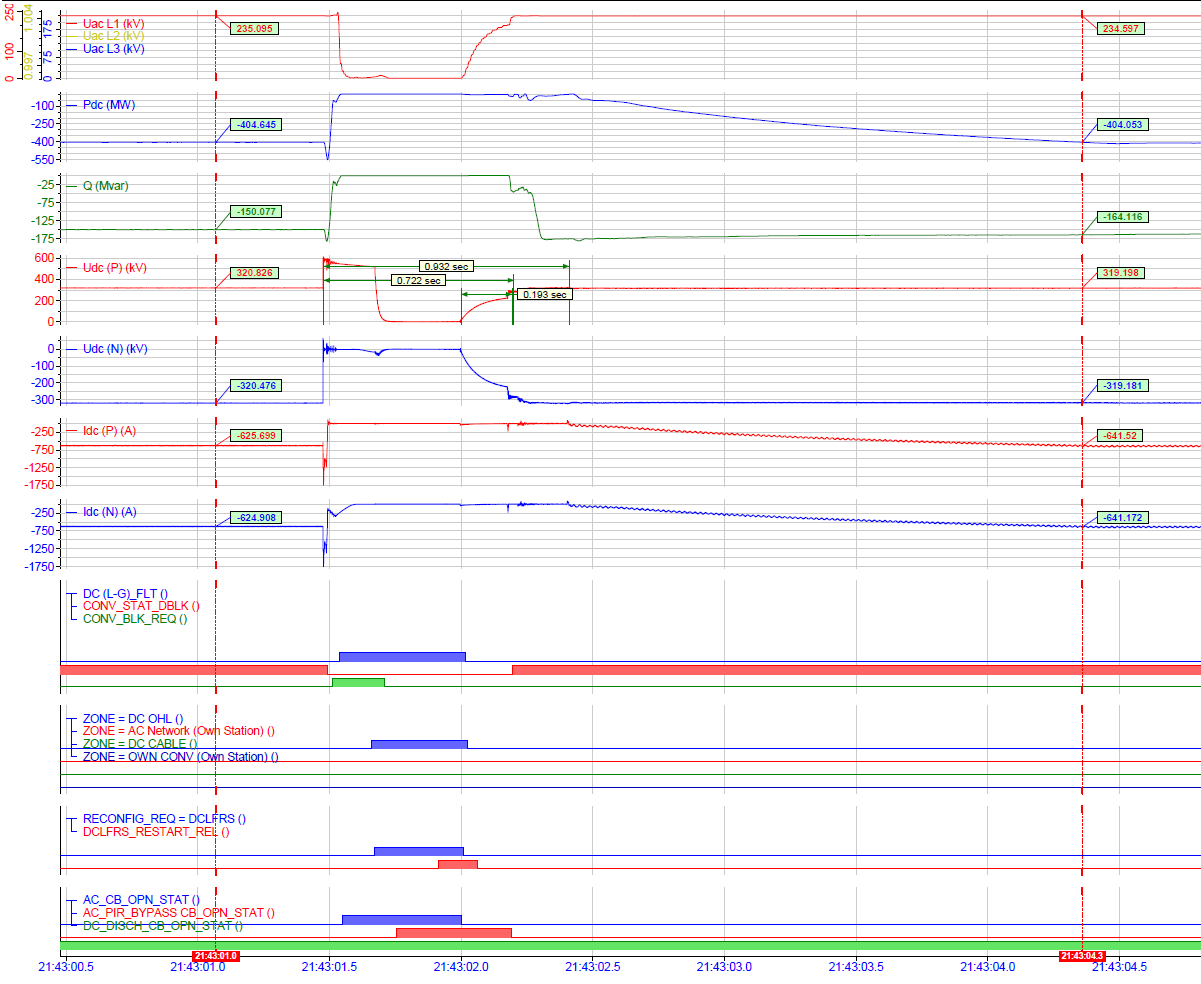
\includegraphics[width=\linewidth]{dc-fault-ride-through/fig/k2026_fig7_tfr_link1_400mw.png}
  \caption{Transient fault record at Pugalur of the pole-to-ground fault on
           the negative pole of link~1 at 400\,MW; from top: AC phase-to-ground
           voltages at the interface transformer, active power, reactive
           power, positive and negative pole voltages, positive and negative
           pole currents, and the binary channels of the protection and the
           switchgear. Reproduced from~[25], Figure~7}
  \label{fig:dcf-pg-tfr}
\end{figure}

\begin{figure}[!ht]
  \centering
  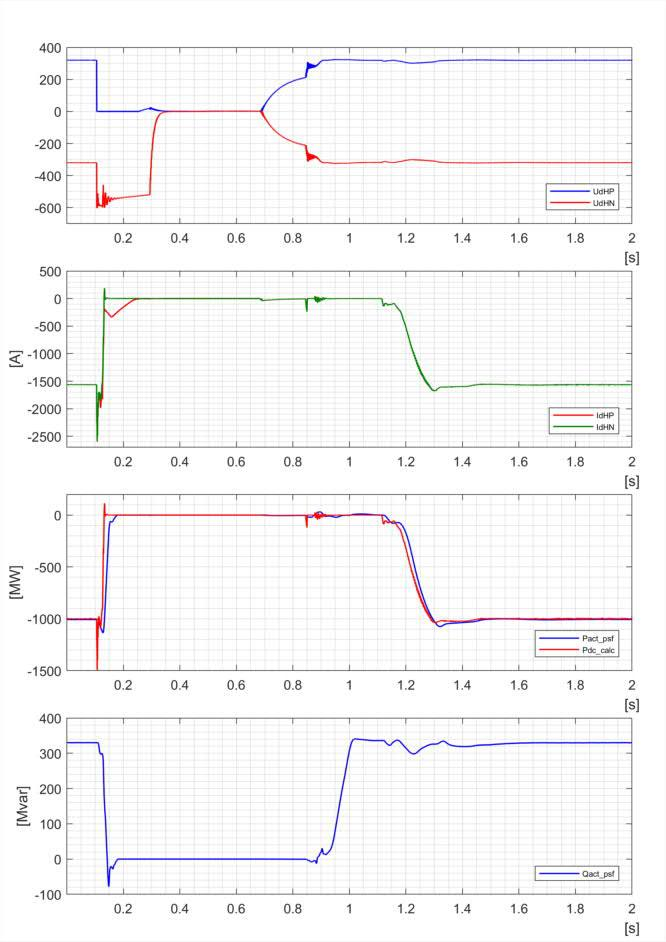
\includegraphics[width=0.6\linewidth]{dc-fault-ride-through/fig/k2026_fig10_simulation_1000mw.png}
  \caption{Dynamic performance study of a pole-to-ground fault on the
           positive pole at 1000\,MW, $+330$\,Mvar; from top: pole voltages,
           pole currents, active power and reactive power. Reproduced
           from~[25], Figure~10}
  \label{fig:dcf-simulation}
\end{figure}

\begin{table}[!ht]
  \centering
  \begin{tabular}{@{}l r r r l r r@{}}
    \toprule
    \textbf{Case} & \multicolumn{1}{c}{$P$} & \multicolumn{1}{c}{$Q$}
      & \multicolumn{1}{c}{\textbf{Current}} & \multicolumn{1}{c}{\textbf{Faulted pole}}
      & \multicolumn{1}{c}{\textbf{Deblock}} & \multicolumn{1}{c}{\textbf{Power}} \\
      & \multicolumn{1}{c}{MW} & \multicolumn{1}{c}{Mvar} & \multicolumn{1}{c}{A}
      & & \multicolumn{1}{c}{ms} & \multicolumn{1}{c}{s} \\
    \midrule
    Link~1, field       &  400 & $-150$ &  625 & negative & 930 & 2 \\
    Link~2, field       &  250 &    0   &  390 & positive & 890 & 2 \\
    Link~2, field       &  400 &    0   &  625 & negative & 860 & 2 \\
    Simulation, rated   & 1000 & $+330$ & 1563 & positive & $< 800$ & $\approx 2$ \\
    \bottomrule
  \end{tabular}
  \caption{Recorded and simulated first restarts after a pole-to-ground
           fault on the Pugalur--Thrissur link, reverse power flow Thrissur to
           Pugalur; deblocking time after $t_0$ and time to pre-fault
           power~[25]}
  \label{tab:dcf-events}
\end{table}

\subsubsection{Pole-to-pole fault}
\label{sec:dc-fault-records-pp}

The commissioning record of a pole-to-pole fault in~[24] shows the fault
current fed through the diode rectifiers after blocking, with the
corresponding reactive power drawn from the AC network as for a three-phase
fault with residual voltage. After the circuit breakers open the current
decays and reaches zero in both stations at $t_0 + 145$\,ms. The circuit
breakers reclose at $t_0 + 850$\,ms and passive charging begins; station~A
deblocks at $t_0 + 1.03$\,s and station~B at $t_0 + 1.25$\,s, with the same
restart procedure as after a pole-to-ground fault. The sequence contains no
discharge step, but it has to allow for the current decay of up to 500\,ms,
Section~\ref{sec:dc-fault-behaviour}, and for the deionisation time after
it before the circuit breakers reclose~[24]. Figure~\ref{fig:dcf-pp-record}
is the record: both pole voltages collapse to zero without overvoltage, the
pole currents peak at about $-10$\,kA before the breakers open, and the
reactive power of both stations shows the three-phase fault seen from the
AC side.

\begin{figure}[!ht]
  \centering
  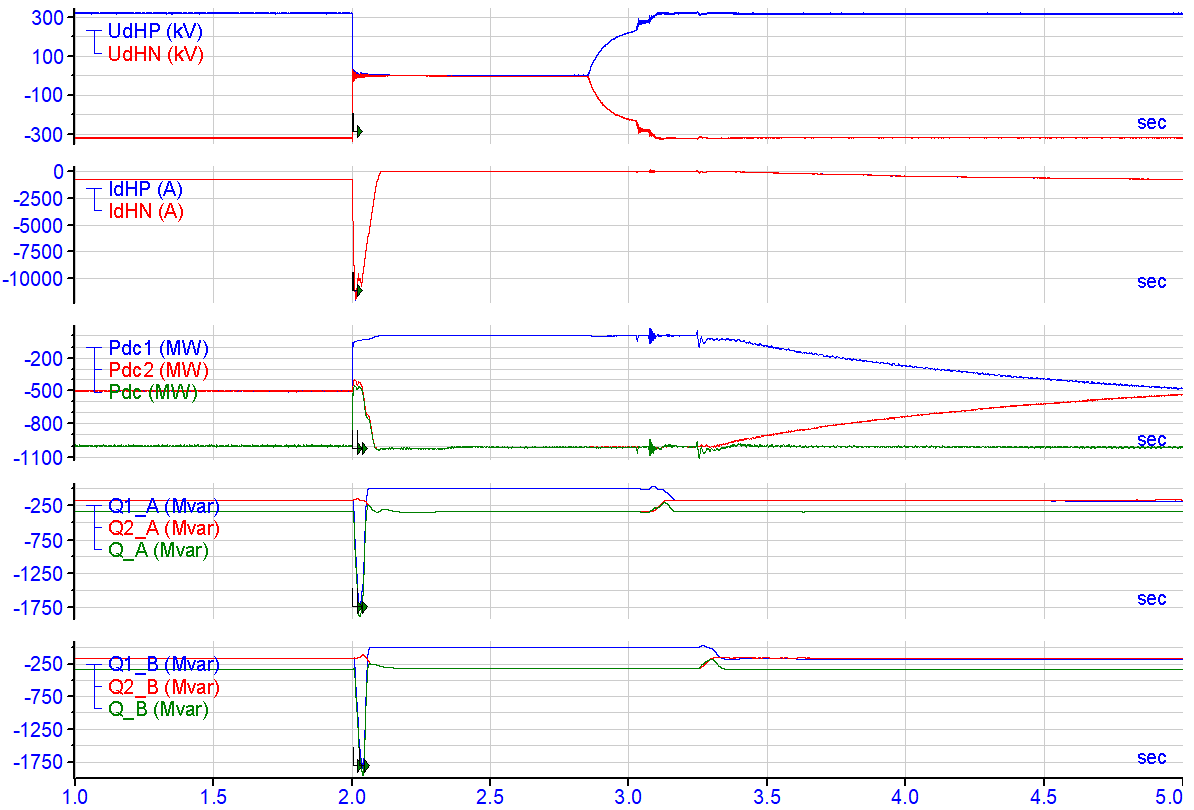
\includegraphics[width=\linewidth]{dc-fault-ride-through/fig/w2022_fig4_pp_recovery.png}
  \caption{Commissioning record of the first restart after a pole-to-pole
           fault on link~1; from top: pole voltages, pole currents, active
           power of link~1, link~2 and total, reactive power at station~A and
           at station~B. Reproduced from~[24], Figure~4}
  \label{fig:dcf-pp-record}
\end{figure}

\subsubsection{Recovery at reduced direct voltage}
\label{sec:dc-fault-records-reduced}

The second restart recovers to a reduced direct voltage. A half-bridge MMC
has a narrow direct-voltage range: to avoid over-modulation, the direct
voltage to ground has to stay above the peak of the AC voltage the converter
produces at its terminals, so the AC-side voltage has to be lowered with the
direct voltage. The ratio of the interface transformer is changed with its
on-load tap-changer, before the circuit breaker recloses, since the link has
to recover to the reduced voltage immediately after deblocking. Depending on
the number of taps this takes up to 1\,min~[24]. The operator preselects the
reduced voltage between $\pm$256\,kV and $\pm$305\,kV; a link already
running below the preselected level is kept from being raised to it by the
recovery~[24]. The commissioning record of a second restart from
$\pm$320\,kV to $\pm$256\,kV, with the other link out of service, shows the
power restored about 60\,s after the fault~[24],
Figure~\ref{fig:dcf-reduced-record}; the time axis of that record spans
70\,s, against 4\,s for the first restarts of
Figures~\ref{fig:dcf-pg-record} and~\ref{fig:dcf-pp-record}.

\begin{figure}[!ht]
  \centering
  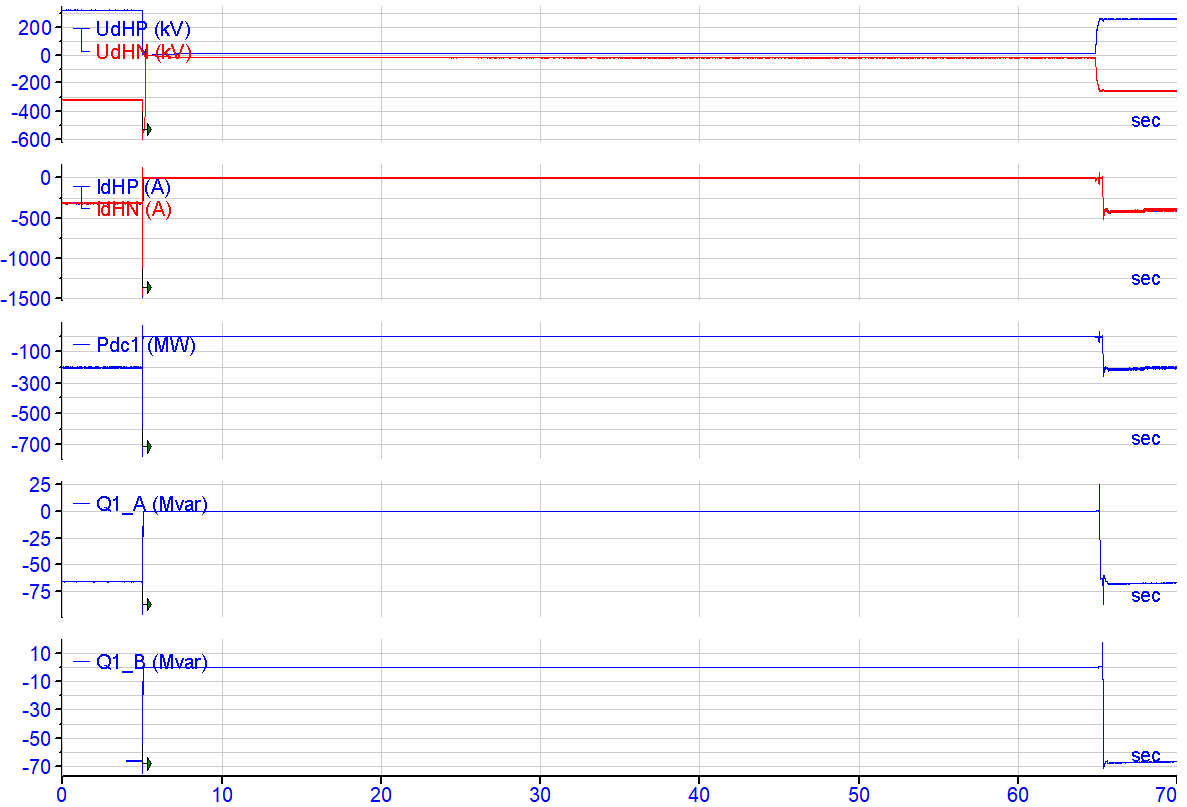
\includegraphics[width=\linewidth]{dc-fault-ride-through/fig/w2022_fig5_reduced_voltage.png}
  \caption{Commissioning record of a second restart to the reduced direct
           voltage of $\pm$256\,kV after a pole-to-ground fault, other link
           out of service; from top: pole voltages, pole currents, active
           power of link~1, reactive power at station~A and at station~B.
           Reproduced from~[24], Figure~5}
  \label{fig:dcf-reduced-record}
\end{figure}

\subsection{Fault zones and selectivity}
\label{sec:dc-fault-zones}

A restart is permitted only for a fault on the overhead line. The protection
of each link is therefore divided into the fault zones AC network, converter
station, DC overhead line and DC cable at each end, Figure~\ref{fig:dcf-zones},
with the HVDC link zone spanning both converters and the DC
circuit~[24], [25]. Voltage and current measurements at the zone
boundaries --- current transformers at the transition station separate the
overhead line from the cable --- produce fault zone identifiers that state
on which side of the measuring point the fault lies. A logic combines the
identifiers from all locations while the fault clearing is in progress, so
that the zone is known before the recovery sequence is released~[24]. On the
Pugalur records the zone identification and the reconfiguration request fall
into the discharge phase, before $t_0 + 250$\,ms~[25].

Two identifier algorithms cover the range of fault impedances an overhead
line produces~[24]. Faults of low impedance are detected by a wave-front
logic that evaluates the polarity of the instantaneous changes of the direct
current. Faults of high impedance are detected by a residual-current logic
acting on the discharge currents of the DC cable; it covers fault impedances
up to 5\,k$\Omega$.

\begin{figure}[!ht]
  \centering
  \begin{tikzpicture}[font=\footnotesize, >=Latex, line width=0.7pt]
    % AC networks
    \draw[pattern=north east lines, pattern color=atBorderStrong] (0,-0.5) rectangle (0.9,0.5);
    \draw[pattern=north east lines, pattern color=atBorderStrong] (12.1,-0.5) rectangle (13.0,0.5);
    % station A
    \draw (0.9,0) -- (1.6,0);
    \draw (1.6,0) -- (2.1,0.25);
    \draw (2.15,0) -- (2.6,0);
    \draw (2.85,0) circle (0.25); \draw (3.2,0) circle (0.25);
    \draw (3.45,0) -- (3.8,0);
    \draw (3.8,-0.6) rectangle (4.9,0.6); \draw (3.8,-0.6) -- (4.9,0.6);
    \node at (4.05,0.3) {$\approx$}; \node at (4.65,-0.3) {$=$};
    % DC circuit
    \draw (4.9,0.35) -- (8.1,0.35); \draw (4.9,-0.35) -- (8.1,-0.35);
    \draw[line width=2.2pt] (6.9,0.35) -- (8.1,0.35);
    \draw[line width=2.2pt] (6.9,-0.35) -- (8.1,-0.35);
    % station B
    \draw (8.1,-0.6) rectangle (9.2,0.6); \draw (8.1,-0.6) -- (9.2,0.6);
    \node at (8.35,0.3) {$\approx$}; \node at (8.95,-0.3) {$=$};
    \draw (9.2,0) -- (9.55,0);
    \draw (9.8,0) circle (0.25); \draw (10.15,0) circle (0.25);
    \draw (10.4,0) -- (10.9,0);
    \draw (10.9,0) -- (11.4,0.25);
    \draw (11.45,0) -- (12.1,0);
    % zone boundaries
    \foreach \x in {1.3, 5.6, 6.9, 8.6, 11.7} {
      \draw[atDanger, dashed, line width=0.6pt] (\x,-1.0) -- (\x,1.0);
    }
    % zone labels
    \draw[<->, atFgMuted] (0.0,-1.25) -- (1.3,-1.25) node[midway, below, text=atFg] {AC network A};
    \draw[<->, atFgMuted] (1.3,-1.25) -- (5.6,-1.25) node[midway, below, text=atFg] {converter station A};
    \draw[<->, atFgMuted] (5.6,-1.25) -- (6.9,-1.25) node[midway, below, text=atFg] {DC OHL};
    \draw[<->, atFgMuted] (6.9,-1.25) -- (8.6,-1.25) node[midway, below, text=atFg] {DC cable};
    \draw[<->, atFgMuted] (8.6,-1.25) -- (11.7,-1.25) node[midway, below, text=atFg] {converter station B};
    \draw[<->, atFgMuted] (11.7,-1.25) -- (13.0,-1.25) node[midway, below, text=atFg] {AC network B};
    \draw[<->, atFgMuted] (1.3,1.25) -- (11.7,1.25) node[midway, above, text=atFg] {HVDC link zone};
  \end{tikzpicture}
  \caption{Fault zones of one link of the Pugalur--Thrissur project, after~[24],
           [25]; the thick section is the DC cable between the transition
           station and station~B}
  \label{fig:dcf-zones}
\end{figure}

\subsection{Reconfiguration to STATCOM operation}
\label{sec:dc-fault-statcom}

The outcome of each attempt is classified by the passive charging and the
following 15\,min~[24]. A fault detected anywhere in the link during a
restart attempt makes the fault \emph{permanent}, and no further attempt
follows: on a persisting pole-to-ground fault the direct voltage builds up
in one pole only after the circuit breaker closes, the current stays limited
by the insertion resistor, the protection detects the condition, the
start-up is aborted and the healthy pole is discharged,
Figure~\ref{fig:dcf-permanent}. An attempt is
\emph{successful} when the power is restored; a fault after that point is
\emph{consecutive} and starts the next attempt. When 15\,min pass without a
fault the sequence is complete.

\begin{figure}[!ht]
  \centering
  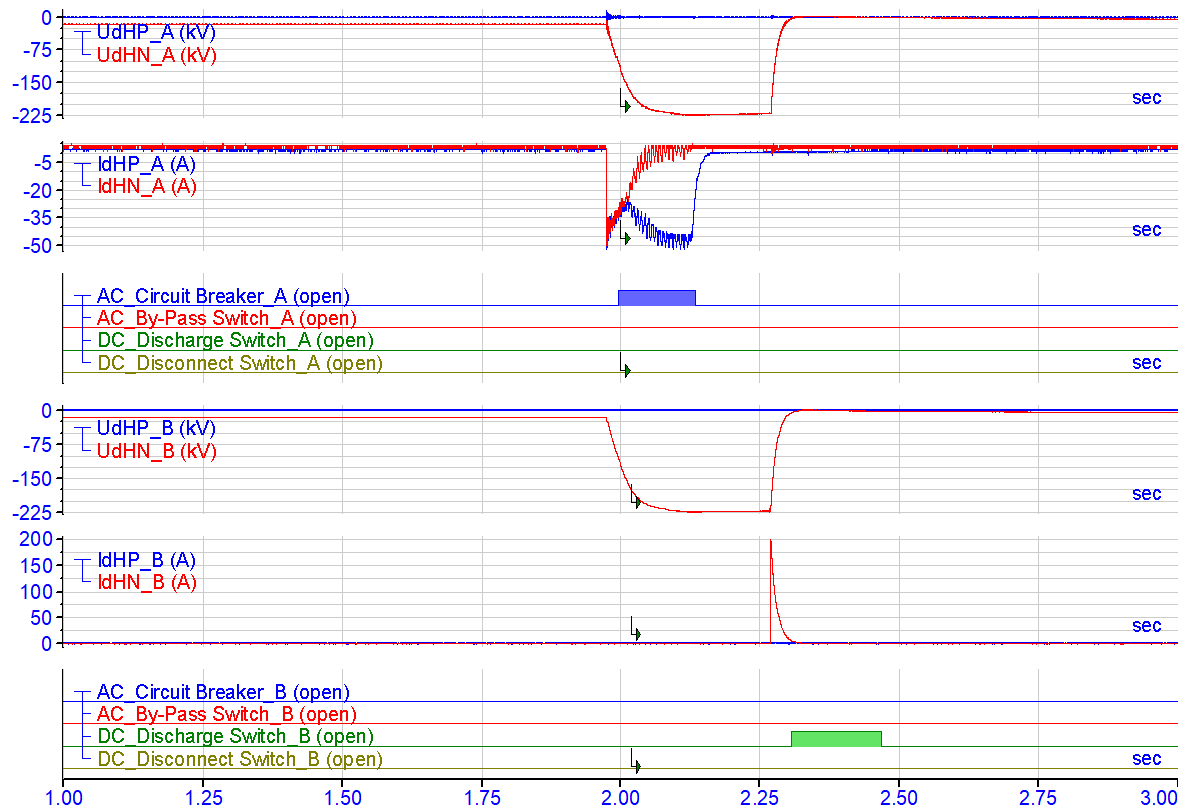
\includegraphics[width=0.9\linewidth]{dc-fault-ride-through/fig/w2022_fig8_permanent_fault.png}
  \caption{Commissioning record of a restart attempt on a permanent
           pole-to-ground fault on the positive pole: after the circuit
           breaker of station~A closes, the voltage builds up in the negative
           pole only, the currents stay limited by the insertion resistor,
           the attempt is aborted and the discharge switch of station~B
           removes the healthy-pole voltage; for each station the pole
           voltages, pole currents and the positions of circuit breaker,
           bypass switch, discharge switch and DC disconnect switch.
           Reproduced from~[24], Figure~8}
  \label{fig:dcf-permanent}
\end{figure}

A sequence ends unsuccessfully either by a permanent fault or by a third
consecutive fault. In both cases both stations change over to STATCOM
operation after the fault clearing: the DC disconnect switches separate each
converter from the DC circuit and each station restarts independently~[24].
The changeover time is the sum of the operating time of the slow DC
disconnect switches and, when the link was running at rated voltage, of the
tap-changer movement to the STATCOM position; it ranges from 15\,s to about
1\,min. In the commissioning record of~[24] the link was already at reduced
voltage, the disconnect switches were the only term, and both stations
restored reactive power within about 14\,s,
Figure~\ref{fig:dcf-statcom-record}. The converters are therefore
unavailable for the transient voltage support in the first seconds after the
loss of transmission and available for the steady-state support afterwards.

The same changeover is started directly, without any restart attempt, when
the fault zone is the DC cable~[24], [25]. A fault in one converter station
prohibits the changeover for that station, and only the other one
reconfigures to STATCOM operation~[24].

\begin{figure}[!ht]
  \centering
  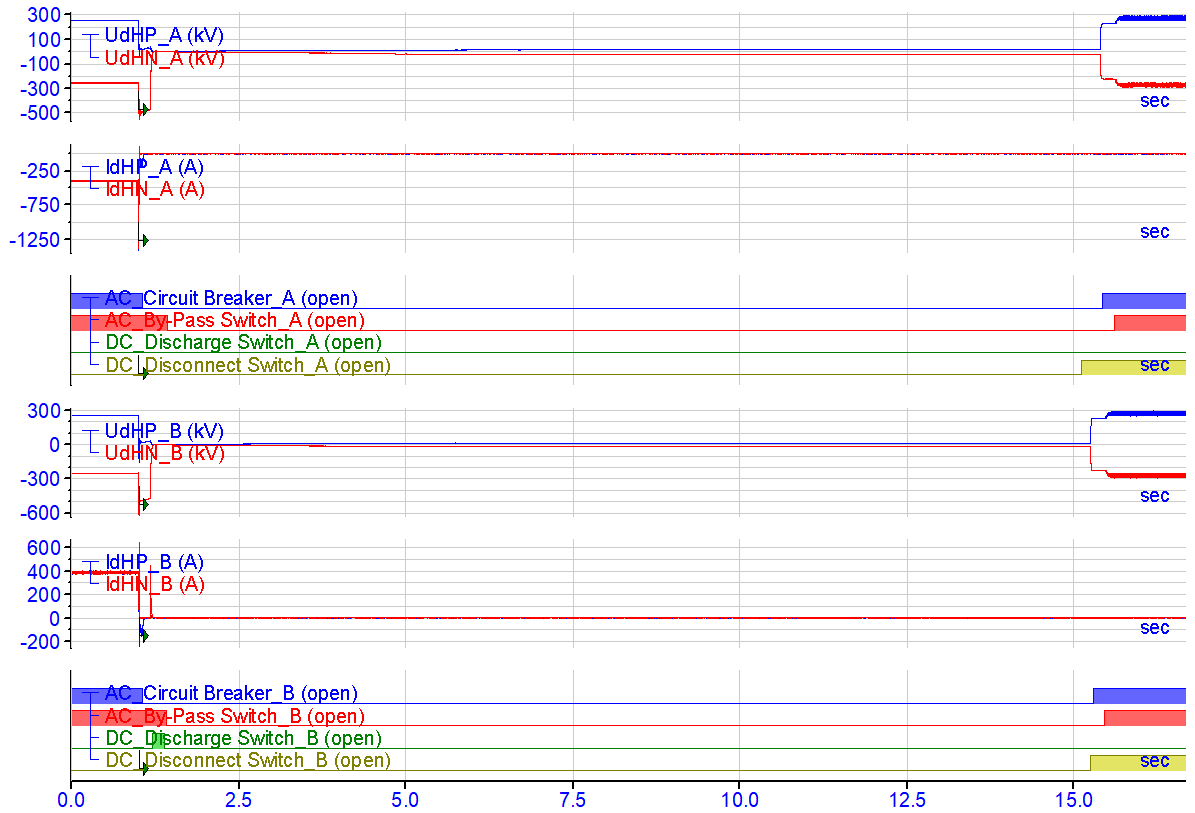
\includegraphics[width=0.9\linewidth]{dc-fault-ride-through/fig/w2022_fig9_statcom_changeover.png}
  \caption{Commissioning record of the changeover to STATCOM operation after
           a third consecutive pole-to-ground fault, link previously at
           reduced direct voltage: the DC disconnect switches open and both
           stations deblock at about 15\,s; for each station the pole
           voltages, pole currents and the switch positions. Reproduced
           from~[24], Figure~9}
  \label{fig:dcf-statcom-record}
\end{figure}

\subsection{Ratings affected by the recovery}
\label{sec:dc-fault-ratings}

The short-circuit level of the AC networks acts in opposite directions on
the two fault types~[24]: the pole-to-pole fault current rises with the
short-circuit level, whereas the pole-to-ground overvoltage rises as the
short-circuit level falls, because the load rejection of the faulted link
raises the AC voltage more in a weak network. The pre-fault active and
reactive power have no comparable influence on the fault behaviour beyond
this overvoltage effect. The commissioning tests of~[24] were run at
short-circuit levels above 10\,GVA and at a pre-fault power the healthy link
could compensate in full. The equipment ratings and the protection settings
were fixed against a defined relation of network overvoltage to
short-circuit level, so that the extreme network conditions are covered
without over-rating~[24].

The cable section raises the fault rate of the DC circuit, since the
overhead line is exposed, while it is the cable that has to carry the fault
currents and the overvoltages~[24]. The currents through the cable screens
and the grounding system, the overvoltages across the main insulation and
the polarity reversals enter the cable rating. Measurements at the Thrissur
cable termination for faults on the overhead line near Pugalur show the
$\mathrm{d}u/\mathrm{d}t$ of the initial voltage collapse reduced by the
cable impedance, a well damped response to the pole-to-ground fault, and a
first voltage reversal of about 40\,\% for the pole-to-pole fault,
Figure~\ref{fig:dcf-cable-stress}; steep fronts lie outside the bandwidth
of the installed recorders and were covered in the design studies~[24].

\begin{figure}[!ht]
  \centering
  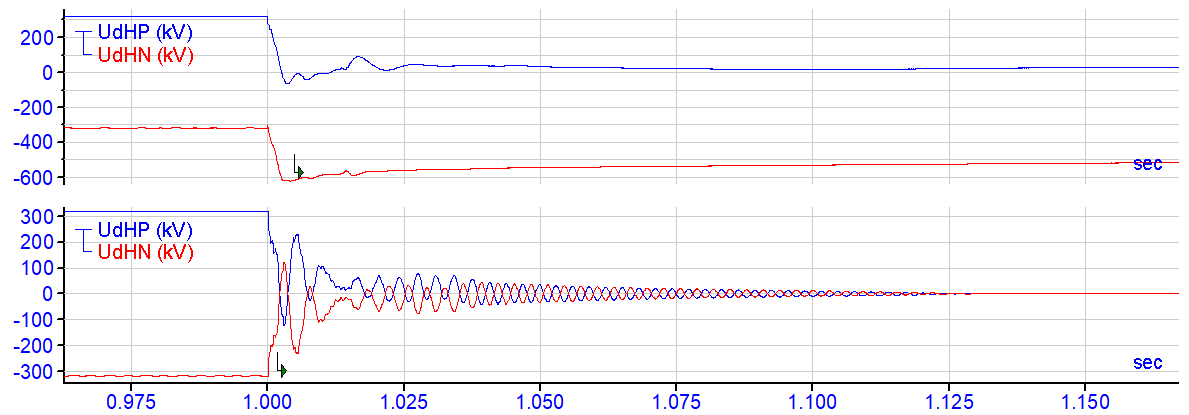
\includegraphics[width=0.9\linewidth]{dc-fault-ride-through/fig/w2022_fig6_cable_stress.png}
  \caption{Pole voltages at the Thrissur cable termination within the first
           150\,ms of a fault on the overhead line near Pugalur: single
           pole-to-ground fault (upper) and pole-to-pole fault (lower).
           Reproduced from~[24], Figure~6}
  \label{fig:dcf-cable-stress}
\end{figure}

Each fault and recovery is a thermal event. The devices with long thermal
time constants --- arresters, insertion and discharge resistors, and the
star-point unit --- are rated for the specified number of recoveries, three
sequences within 45\,min, and their thermal state is monitored by the
protection~[24]. The star-point unit also sets the steady-state grading of
the two pole voltages: the unsymmetrical leakage of a DC overhead line, from
insulator and corona currents, was specified as a maximum grading current
unbalance for this project, and for considerably longer overhead sections
the supplier states that the present grading devices may not remain an
economic solution~[24].

\subsection{Design alternatives}
\label{sec:dc-fault-alternatives}

Four alternatives were evaluated at the offer stage of the project and
rejected on cost~[24].

\begin{itemize}[itemsep=0.2em]
  \item \textbf{Full-bridge sub-modules.} A full-bridge MMC is an open
        circuit when blocked, so the AC circuit breaker need not open and
        the AC network is less disturbed, and it operates at a modulation
        index above one, so it recovers to a reduced direct voltage without
        the tap-changer. Both remove mechanical operations from the sequence
        and shorten the recoveries and changeovers. The alternative was set
        aside for its higher investment and losses, and because few bidders
        could offer it.
  \item \textbf{DC circuit breaker.} Clears the fault in the DC circuit and
        may keep the converters in service. Precautions for the DC
        overvoltage and the cable inrush remain and enter the achievable
        recovery time. Rejected for investment cost and the lack of
        competing bidders.
  \item \textbf{Fixed no-load voltage.} A converter-side no-load voltage
        chosen for the minimum direct voltage at the maximum modulation
        index allows recovery to any direct voltage within the same
        1.5\,s or 1.8\,s, without tap-changer movement. The converter then
        operates at a higher AC current, with operating losses about 20\,\%
        higher. The project chose the losses over the recovery time.
  \item \textbf{Fast disconnect switches.} Would reduce the changeover to
        STATCOM operation to the few seconds of the fault clearing, but only
        when the link was already at reduced voltage, since otherwise the
        tap-changer sets the time; their price is 5 to 10 times that of slow
        disconnects, and the probability of a fast changeover was judged
        low.
\end{itemize}

\subsection{Transfer to a single-link scheme}
\label{sec:dc-fault-single}

The recovery times above hold for the converter type and switchgear
described; the supplier states that a substantial reduction requires a
different converter topology that makes the mechanical switches
unnecessary~[24]. The power compensation during a first restart is specific
to the two-link project: a scheme with one link has no parallel path, and
the loss of transmission until deblocking --- 0.86 to 1.25\,s in the records
of Section~\ref{sec:dc-fault-records} --- and the ramp to pre-fault power
within 2\,s act on the AC network at both ends. For such a project the
supplier names other measures to limit that impact as a requirement~[24].

\FloatBarrier
